\documentclass{standalone}

\usepackage{tikz}

\usetikzlibrary{shapes.geometric}
\begin{document}
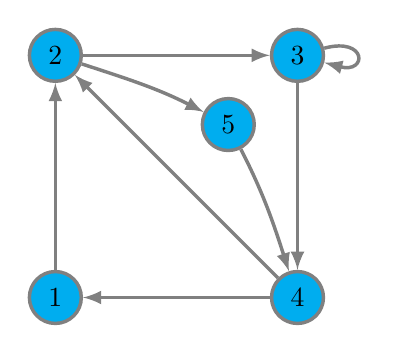
\begin{tikzpicture}
[every node/.style={inner sep=0pt}]
\node (2) [circle, minimum size=18.75pt, fill=cyan, line width=1.25pt, draw=gray] at (50.0pt, -25.0pt) {\textcolor{black}{2}};
\node (5) [circle, minimum size=18.75pt, fill=cyan, line width=1.25pt, draw=gray] at (112.5pt, -50.0pt) {\textcolor{black}{5}};
\node (1) [circle, minimum size=18.75pt, fill=cyan, line width=1.25pt, draw=gray] at (50.0pt, -112.5pt) {\textcolor{black}{1}};
\node (4) [circle, minimum size=18.75pt, fill=cyan, line width=1.25pt, draw=gray] at (137.5pt, -112.5pt) {\textcolor{black}{4}};
\node (3) [circle, minimum size=18.75pt, fill=cyan, line width=1.25pt, draw=gray] at (137.5pt, -25.0pt) {\textcolor{black}{3}};
\draw [line width=1.25, ->, >=latex, color=gray] (1) to  (2);
\draw [line width=1.25, ->, >=latex, color=gray] (2) to  (3);
\draw [line width=1.25, ->, >=latex, color=gray] (3) to  (4);
\draw [line width=1.25, ->, >=latex, color=gray, loop right] (3) to (3);
\draw [line width=1.25, ->, >=latex, color=gray] (4) to  (1);
\draw [line width=1.25, ->, >=latex, color=gray] (4) to  (2);
\draw [line width=1.25, ->, >=latex, color=gray] (2) to  [in=153, out=342] (5);
\draw [line width=1.25, ->, >=latex, color=gray] (5) to  [in=108, out=297] (4);
\end{tikzpicture}
\end{document}
